\chapter{Exploiting The Tools From Theory Code in Fermionic Systems.}
In the last chapter we talked about Fermionic systems and the formalism used when dealing with it. In this chapter we first are going to  mention some concepts and definitions in order to understand how the coding theory can be linked to Fermionic states, particularly we will discuss the case of random minimum codes and well known results about this subject. We will talk about the exponent errors for random minimum codes and we will show how all this theory can be linked to the case Fermionic random minimum codes and compute its correspondent exponent error. 

\section{Error correcting Code Theory}
In 1948, Claude Shannon presents his extraordinary work named ``A Mathematical Theory of Communication'' \cite{shannon_mathematical_1948} in which he provided a precise measure of the information content of a random variable in terms of its entropy.  His work is divided in two parts the noiseless coding theorem and the noisy channel theorem. For the purpose of our needs we are going to focus only in the second part of his work, which states that a reliable communication is possible if we use schemes such that its rate is less than the capacity of the channel. Even though he never provided an idea of how this schemes could be found, his work is considered one of the most relevant discovery of the century.
\begin{figure}
\centering
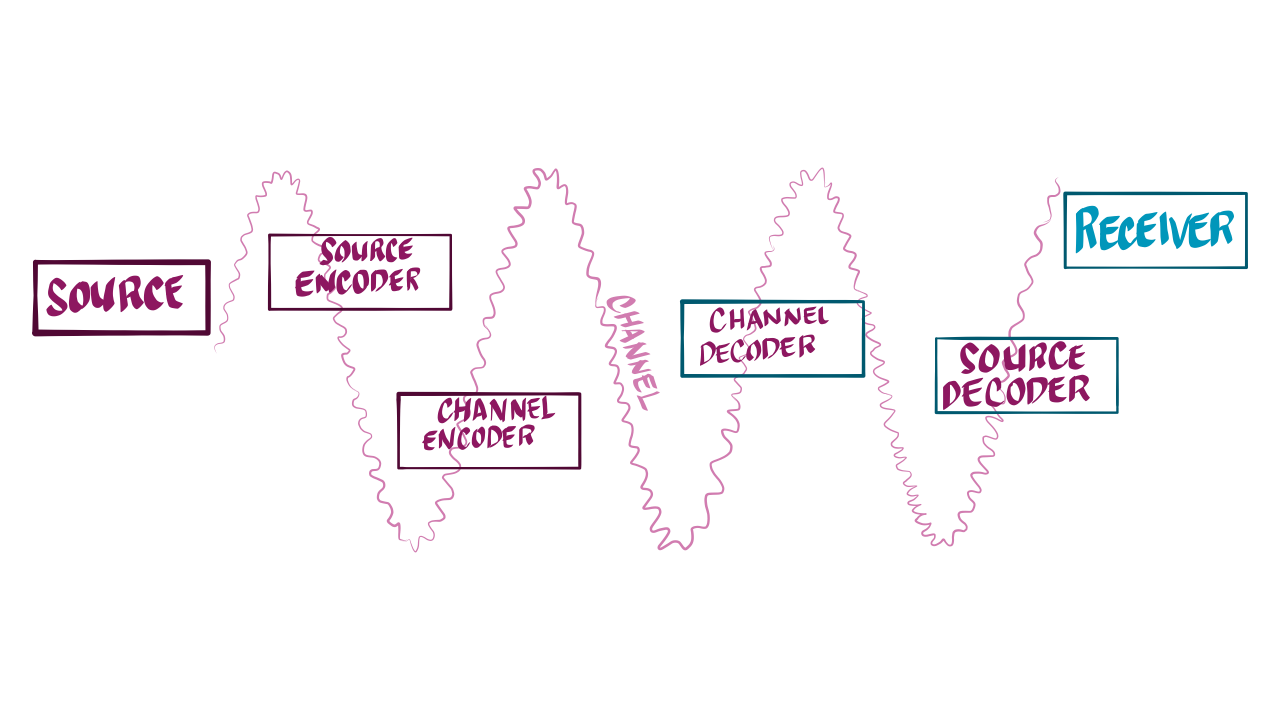
\includegraphics[width=0.9\textwidth]{Figures/Source_Destination.png}
\caption{Representation of the scheme of communication. In the image the noise in the channel is represented by the noise wavy connection between the parts in the communication. }
\label{CH2:Channel_communication}
\end{figure}
\indent Here we will consider codes in communication scenario, as the one showed in figure \ref{CH2:Channel_communication}, meaning that there will be a sender who wants to send $k$ message symbols over a noisy channel and there will be a receiver who has to correct possible errors over the sent code to fully interpret it. The sender will first encodes the $k$ message symbols into $n$ symbols. The receiver then tries to recover the original $k$ message symbols. thus, encoding is the process of adding redundancy and decoding is the process of removing errors and the communication can only be done over the channel\cite{mackay_information_2003}. The most fundamental question one can ask is what will be the relation between the amount of redundancy and the errors that can be corrected, and in order to answer this question we will provide some useful definitions.
\section{Some basic definitions}
\begin{definition}[Code]
A code of block $C$ length $n$ over an alphabet $\Sigma$ is a subset of $\Sigma^n$.  If $|\Sigma|=q$, we say that $C$ is a q-ary code.
\end{definition}
\indent It is worth mention that, associated with a code there is also an encoding map $E$ which maps the message set $\mathcal{M}$, identified in some canonical way with $\{1,2,\ldots,|C|\}$ say, to code words belonging to $\Sigma^N$, and thus we have to understand the code as the image of the encoding map\cite{jaynes_probability_2003}.
\begin{definition}[Dimension of a code]
Given a code $C\subset\Sigma^n$, its dimension is given by
  \begin{equation}
  k \stackrel{\mathrm{def}}{=} \log _{q}|C|,
  \label{CH2:diemnsion_of_code}
  \end{equation}
 \end{definition}
\indent An interesting fact about defining  the dimension of the code in this way is that implicitly it is telling us that when working with codes exponential growth will be always taken into account.\\

\indent We have to provide here a way to measure the amount of redundancy in a given message.
	\begin{definition}[Rate of a code]
	The rate of a code with dimension $k$ and block length $n$ is given by 
	\begin{equation}
		R \stackrel{\text { def }}{=} \frac{k}{n},
		\label{CH2:Rate_of_code}
	\end{equation}
	\end{definition}
\indent This definition is nothing but the average amount of non redundant information each of the $n$ symbols transmitted over the channel.\\ However, an alternative, and more general way of defining this is via the size of the code and the alphabet as
\begin{equation}
R(C)=\frac{\log |C|}{n \log |\Sigma|}.
\end{equation}

\begin{definition}[Hamming distance]
  The Hamming distance between two strings $x$ and $y$ of the same length over a finite alphabet $\Sigma$, denoted $\Delta(x,y)$, is defined as the number of positions at which the two strings differ, i.e, $\Delta(x,y) = |\{i| x_i \neq y_i\}|$. The fractional Hamming distance or relative distance between $x,y\in \Sigma^n$ is given by $\delta(x,y) = \frac{\Delta(x,y)}{n}$.
 \end{definition}
\indent It is trivial to check that the Hamming distance defines a metric on $\Sigma^n$.
\begin{definition}
\textbf{Hamming weight:} The Hamming weight of a string $x$ over alphabet $\Sigma$ is defined as the number of non-zero symbols in the string. More formally, the Hamming weight of a string $\mathcal{W}(x) = |\{i| x_i \neq 0\}|$. Note that $\mathcal{W}(x-y) = \Delta(x,y)$.
\end{definition}
\indent Given a string $x\in\Sigma^{N}$, the Hamming ball of radius $r$ around $x$ is the set $\{y\in\Delta^n | \Delta(x,y)\leq r\}$.\\

\indent The minimum distance, or simply distance, of a code $C$, denoted $\Delta(C)$, is defined to be the minimum Hamming distance between two distinct code words of $C$. That is
\begin{definition}[Minimum distance]
The minimum distance, or simply distance, of a code $C$, denoted $\Delta(C)$, is defined to be the minimum Hamming distance between two distinct code words of $C$. That is
\begin{equation}
\Delta(C)=\min _{c_{1}, c_{2} \in C \atop c_{1} \neq c_{2}} \Delta\left(c_{1}, c_{2}\right).
\end{equation}
In particular, for every pair of distinct code words in $C$ the Hamming Distance between them is at least $\Delta(C)$
\end{definition}

\indent The relative distance of $C$, denoted $\delta(C)$, is the quantity $\frac{\Delta(C)}{N}$, where $N$ is the block length of $C$. Thus any two code words of $C$ differ in at least a fraction $\Delta(C)$.
\begin{definition}[Notation]
 A q-ary code of block length $N$ and dimension $k$ will be referred to as an $[N,k]_q$ code. Further, if the code has minimum distance $d$, it will be referred to as an $[N,k,d]_q$ code. When the alphabet size $q$ is clear from the context, or not very relevant to the discussion, we omit the subscript.
\end{definition}

\indent Up to this point we have only described specific codes, codes with fixed block length and dimension. However, since we are interested in the asymptotic behaviour, it turns out to be more useful the study of families of codes instead of an specific code.

\begin{definition}[Family of Codes]
 Let $q\geq 2$. let $\{n_i\}_{i\geq 1}$ be and increasing sequence of block lengths and suppose there exists sequences $\{k_i\}_{i\geq 1}$ and $\{d_i\}_{i\geq 1}$ such that for all $i\geq 1$ there exist an $[n_i,k_i,d_i]_q$ code $C_i$. then the sequence $C=\{C_i\}_{i\geq1}$ is a family of codes. The rate of C is defined as
\begin{equation}
R(C)=\lim _{i \rightarrow \infty}\left\{\frac{k_{i}}{n_{i}}\right\},
\label{CH2:Rate_of_family_code}
\end{equation}
and the relative distance of $C$ is defined as
\begin{equation}
\delta(C)=\lim _{i \rightarrow \infty}\left\{\frac{d_{i}}{n_{i}}\right\},
\label{CH2:Relative_distance_of_family_code}
\end{equation}
from now on whenever we talk about a code we are implicitly referring to a family of codes.
\end{definition}
\indent For the purpose of this work, we are going to focus on a particular class of codes, name minimum distance code. This special kind of codes came to our interest since they seem to appear naturally when study typical Fermionic states. We will then show some of the main results on this particular kind of codes to after show how this results could be extended to our particular case.\\

\indent When we talk about codes of minimum distance $d$ we refer to codes which have the property that for every pair $x,y$ of codewords we have that
\begin{equation}
\Delta(x,y) =d,
\end{equation}

and therefore, the its relative distance $\delta$ is given by $N\delta=d$.\\

\indent When working with this kind of codes one may wonder what is the best rate we can achieve. Particularly we are going to show 3 results, 1 positive and 2 negative results\footnote{Note that a negative result refer to an upper bound on the rate, meaning that the maximum achievable rate we could get can not exceed some value. Whereas a positive result refer to  lower bound on the rates we can achieve.}. Even though there are other known bounds, we will not talk about others but Gilbert-Varshamov, Hamming and Plotkin bounds, the reason for this is due to the fact that the other bound apply for large enough alphabets, so for binary codes we are not interested at all in these kind of bounds\cite{mackay_information_2003}.
\begin{figure}
\centering
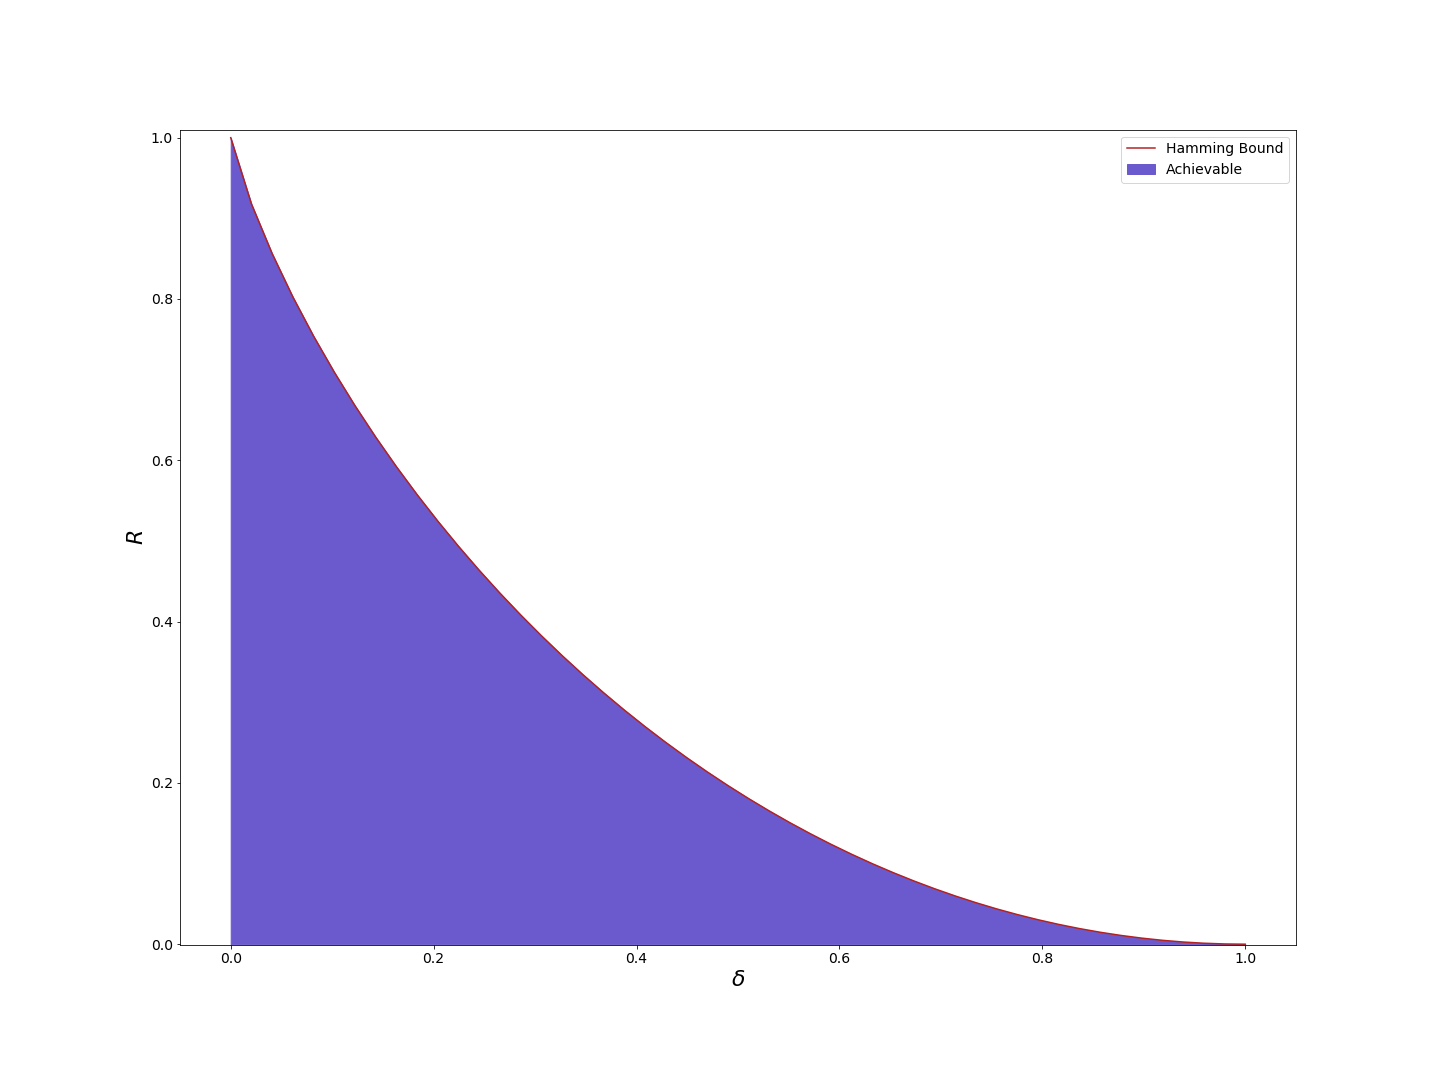
\includegraphics[width=0.7\textwidth]{Figures/Hamming_bound.png}
\caption{An illustration of the Hamming bound for the case of $q=2$. Note any code above this bound could exist. The shaded region shows the codes that could exist.  }
\end{figure}
\subsection{Hamming Bound (Sphere packing bound)}
\begin{definition}[Volume of Hamming ball]
\indent Let $ q\geq2$ and $n \geq r \geq 1$ be integers. Then the volume of a Hamming ball of radius $r$ is given by
\begin{equation}
\operatorname{Vol}_{q}(r, n)=\left|B_{q}(\mathbf{0}, r)\right|=\sum_{i=0}^{r}\left(\begin{array}{l}
n \\
i
\end{array}\right)(q-1)^{i},
\label{CH2:Hamming_ball}
\end{equation}
where the choice of $\mathbf{0}$ as the center of the Hamming ball is chosen arbitrary, since the volume of the Hamming ball is independent of its center.
\end{definition}
\indent It is simple to show that
\begin{equation}
\frac{k}{n} \leq 1-\frac{\log _{q} \operatorname{Vol}_{q}\left(\left\lfloor\frac{d-1}{2}\right\rfloor, n\right)}{n},
\label{CH2:Hamming_bound_1}
\end{equation}
where the volume in \eqref{CH2:Hamming_bound_1} correspond to the definition in\eqref{CH2:Hamming_ball}. With some algebra and using the Stirling asymptotic approximation one can show that
\begin{equation}
\operatorname{Vol}_{q}\left(\left\lfloor\frac{d-1}{2}\right\rfloor, n\right) \geq q^{H_{q}\left(\frac{\delta}{2}\right) n-o(n)},
\end{equation}
where the latter inequality immediately provide us an upper bound on the rate
\begin{equation}
R \leq 1-H_{q}\left(\frac{\delta}{2}\right)+o(1).
\label{CH2:Hamming_bound_2}
\end{equation}

\indent The inequality in \eqref{CH2:Hamming_bound_2} is known as the Hamming Bound.

\subsection{Plotkin Bound}
\begin{definition}[Plotkin Bound]
The following holds for any code $\mathcal{C}\subset [q]^n$ 
\begin{itemize}
\item If $d=\left(1-\frac{1}{q}\right) n,|\mathcal{C}| \leq 2 q n$.
\item If $d>\left(1-\frac{1}{q}\right) n,|\mathcal{C}| \leq \frac{q d}{q d-(q-1) n}$.
\end{itemize}
Note that the Plotkin Bound implies that a code with relative distance $\delta\geq 1-1/q$, must necessarily have $R=0$.
\end{definition}

\begin{definition}
For any q-ary code with relative distance $0 \leq \delta \leq 1-\frac{1}{q}$,
\begin{equation}
R \leq 1-\left(\frac{q}{q-1}\right) \delta+o(1).
\label{CH2:Plotkin_bound}
\end{equation}
\end{definition}

\begin{figure}
\centering
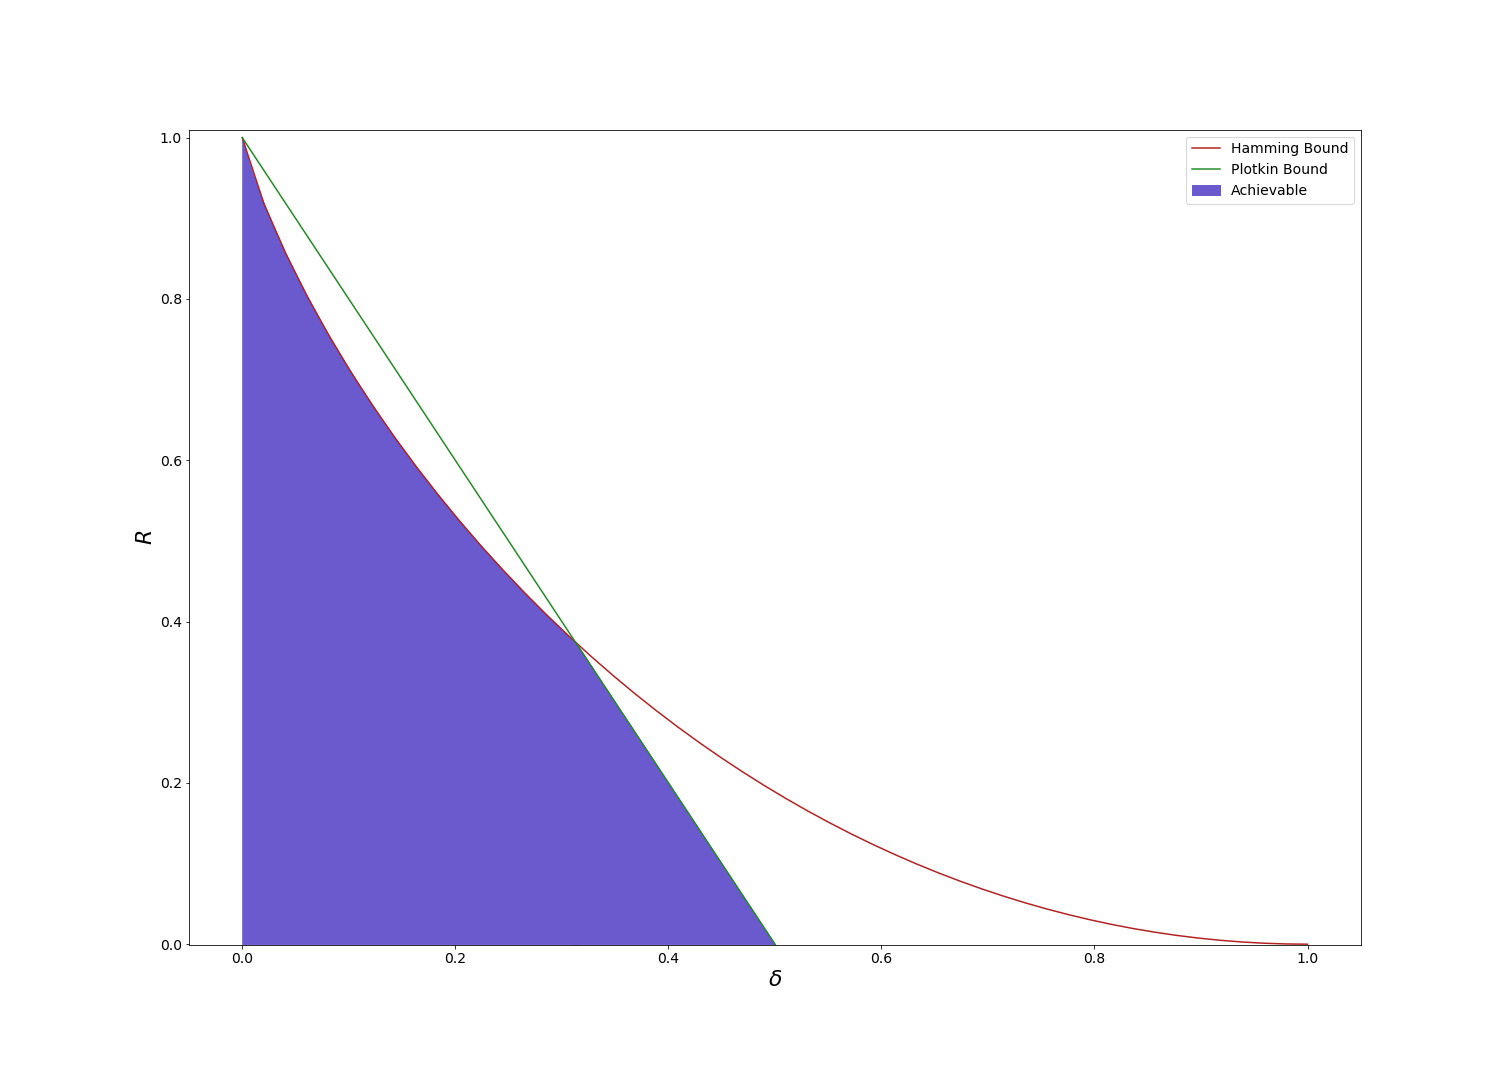
\includegraphics[width=0.7\textwidth]{Figures/Hamming_plotkin_bound.png}
\caption{An illustration of Plotkin and Hamming bounds for the case of $q=2$.  For this case the shaded region changes indicating us that there are not codes with $R>0$ when $\delta=1-1/q$ .}
\end{figure}

\indent To illustrate the proof of this bound we can consider the distance $d=n\delta$. So we can shorten the codewords and group them in a way such that they agree on the first $n-n'$ symbols, with $n^{\prime}=\left\lfloor\frac{q d}{q-1}\right\rfloor-1$. Then in particular for any $x\in [q]^{n-n'}$, define the prefix code
\begin{equation}
\mathcal{C}_{\mathbf{x}}=\left\{\left(c_{n-n^{\prime}+1}, \ldots c_{n}\right) \mid\left(c_{1} \ldots c_{N}\right) \in \mathcal{C},\left(c_{1} \ldots c_{n-n^{\prime}}\right)=\mathbf{x}\right\}.
\end{equation}
for all $x,\ \mathcal{C}_{x}$, has distance $d$ as $\mathcal{C}$ has distance $d$. Additionally, it has block length $n^{\prime}<\left(\frac{q}{q-1}\right) d$, and thus $d>\left(1-\frac{1}{q}\right) n^{\prime}$. From the Plotkin bound, this implies that
\begin{equation}
\left|\mathcal{C}_{\mathbf{x}}\right| \leq \frac{q d}{q d-(q-1) n^{\prime}} \leq q d,
\end{equation}
where the second inequality follows from the fact that $q d-(q-1) n^{\prime}$ is an integer.\\

\indent Note that from the definition of $\mathcal{C}_{x}$
\begin{equation}
|\mathcal{C}|=\sum_{\mathbf{x} \in[q]^{n-n^{\prime}}}\left|\mathcal{C}_{\mathbf{x}}\right|,
\end{equation}
which tell us that 

\begin{equation}
\left.|\mathcal{C}| \leq \sum_{\mathbf{x} \in[q]^{n-n^{\prime}}} q d=q^{n-n^{\prime}} \cdot q d \leq q^{n-\frac{q}{q-1} d+o(n)}=q^{n\left(1-\delta \cdot \frac{q}{q-1}+o(1)\right)}\right.,
\end{equation}

in other words this provides another upper bound to the rate given by
\begin{equation}
R \leq 1-\left(\frac{q}{q-1}\right) \delta+o(1)
\label{CH2:Plotkin:bound_rate}
\end{equation}
\indent To close this part we will show the latter but positive result which provide us  lower bound on the code rates, Gilbert Varshamov bound.
\subsection{Gilbert Varshamov Bound}
We now switch gears to provide a positive result. We will only provide the main ideas for the proof of this result an we will discuss why this result turn out to be one of the most important results.
\begin{definition}[Gilbert-Varshamov Bound]
Let $q\geq 2$. For every $0 \leq \delta<1-\frac{1}{q}$ and $0<\varepsilon \leq 1-H_{q}(\delta)$. There exist a code with rate $R \geq 1-H_{q}(\delta)-\varepsilon$ and relative distance $\delta$.
\label{CH2:Definition_Gilbert_Varshamov}
\end{definition}

\begin{figure}
\centering
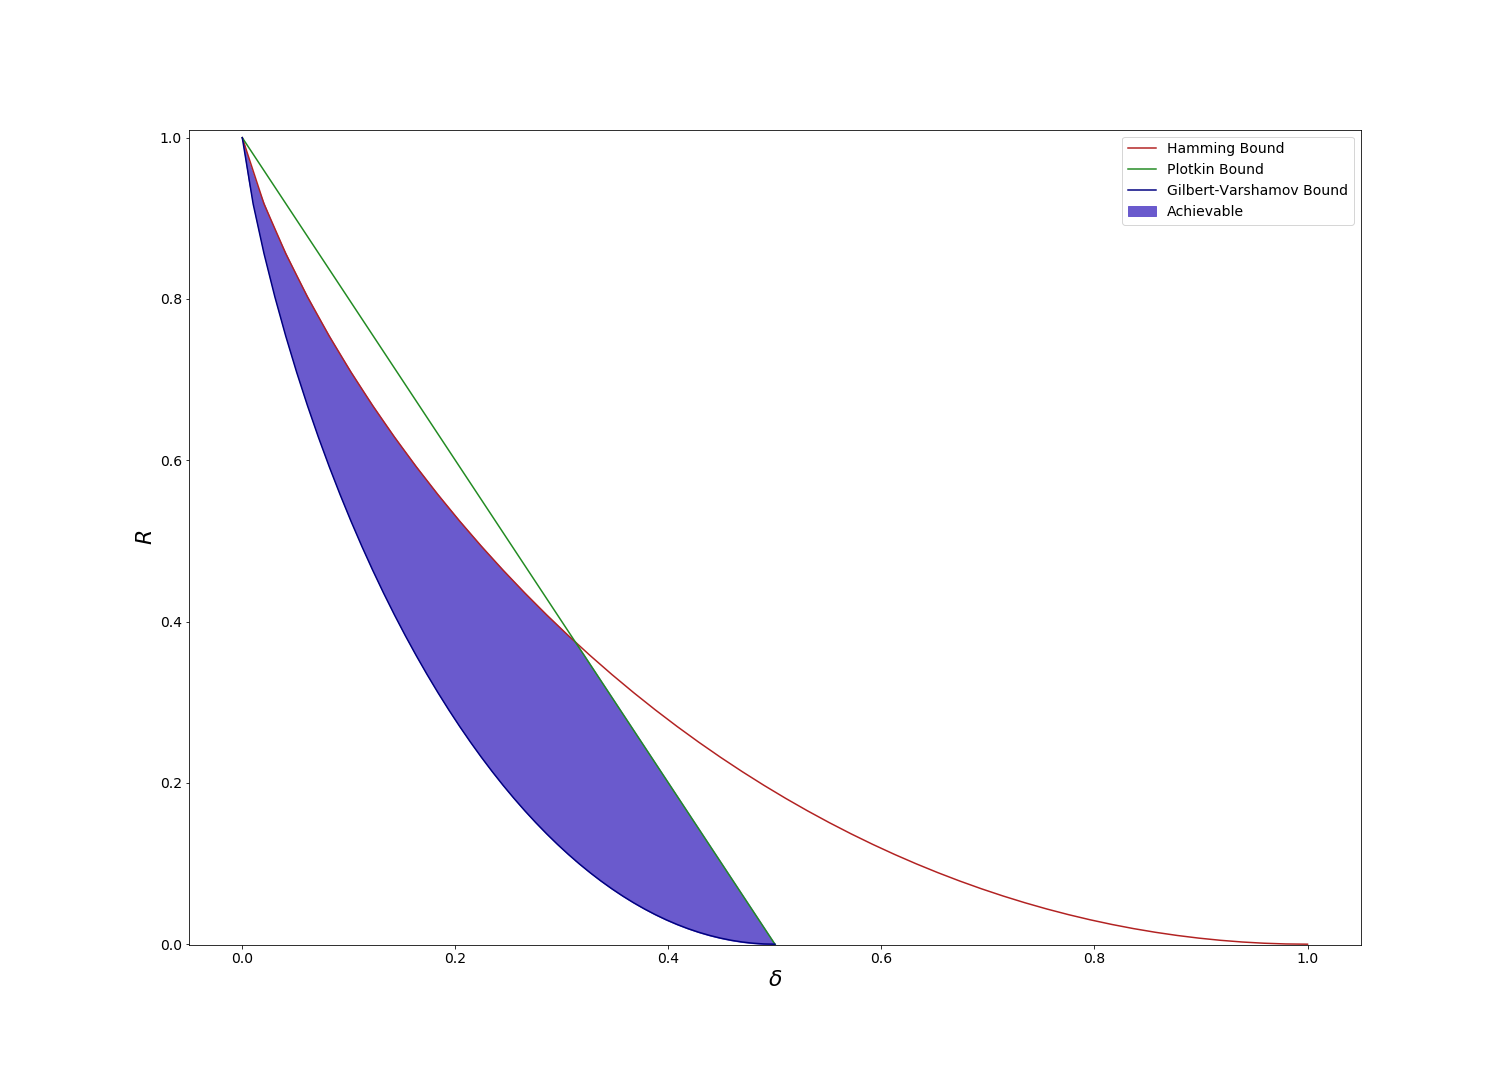
\includegraphics[width=0.7\textwidth]{Figures/Hamming_plotkin_Gilbert_bound.png}
\caption{An illustration of 3 bounds Hamming, Plotkin and Gilbert-Varshamov for the case of $q=2$. The lower bound correspond to the Gilvert-Varshamov Bound whereas the other 2 are the upper bound for the rate.}
\end{figure}

\indent To provide a main idea about the proof we can consider a greedy approach. First we start with an empty code $\mathcal{C}$ and we keep adding vectors that are not in $\mathcal{C}$ and that have Hamming distance at least $d$ from all the existing codewords in $\mathcal{C}$. Notice that by doing so we can assure that we will never add a vector $c$ that will make that will make the distance of $\mathcal{C}$ fall below $d$. Indeed it is easy to see that after doing so, we have
\begin{equation}
\bigcup_{\mathbf{c} \in C} B(\mathbf{c}, d-1)=[q]^{n},
\label{CH2:Gilbert_Varshamov_1}
\end{equation}
this is easily checked, because if it was not true, then there would exist a vector $\mathbf{v} \in[q]^{n} \backslash C$, such that $\Delta(\mathbf{v}, \mathbf{c}) \geq d$ and therefore $\mathbf{v}$ can be added. How ever, this would contradict the fact that we have finished the procedure. So

\begin{equation}
\bigcup_{c \in C} B(\mathbf{c}, d-1) \mid=q^{n}.
\label{CH2:Gilbert_Varshamov_2}
\end{equation}
It isn't hard to see that
\begin{equation}
\sum_{\mathbf{c} \in C}|B(\mathbf{c}, d-1)| \geq\left|\bigcup_{\mathbf{c} \in C} B(\mathbf{c}, d-1)\right|,
\label{CH2:Gilbert_Varshamov_3}
\end{equation}

which implies that
\begin{equation}
\sum_{\mathbf{c} \in C}|B(\mathbf{c}, d-1)| \geq q^{n},
\label{CH2:Gilbert_Varshamov_4}
\end{equation}
but as mentioned before, the volume of the Hamming ball is translation invariant,

\begin{equation}
\sum_{\mathbf{c} \in C} \operatorname{Vol}_{q}(d-1, n) \geq q^{n}.
\label{CH2:Gilbert_Varshamov_5}
\end{equation}

Since $\sum_{\mathbf{c} \in C} V o l_{q}(d-1, n)=V o l_{q}(d-1, n) \cdot|C|$ 

\begin{equation}
\begin{aligned}
|C| & \geq \frac{q^{n}}{\operatorname{Vol}_{q}(d-1, n)} \\
& \geq \frac{q^{n}}{q^{n H_{q}(\delta)}} \\
&=q^{n\left(1-H_{q}(\delta)\right)}.
\end{aligned}
\label{CH2:Gilbert_Varshamov_final}
\end{equation}

\indent Therefore concluding the proof. It is worth mention that this way of proceeding the code have not any special structure but as one might think this algorithm will take exponentially long time to finish. How ever, one may wonder if there is a special kind of code that also achieve this rate. Indeed is possible to show that random linear codes lies, with high probability, on the Gilbert-Varshamov Bound. To pick a linear random code we only need pick a random $k\times n $ matrix, in which each entry is chosen uniformly and independently at random according to its alphabet\cite{mackay_information_2003,jaynes_probability_2003}. Aside from these result providing some bounds on the rate of the minimum distance codes. We are interested in the performance of a special kind of random codes, more specifically binary codes over a binary-symmetric channel (BSC). In here we derive the minimum distance, distance distribution and error exponent of a typical random code (TRC) from a random code ensemble (RCE), as well as the one correspondent to a typical linear code (TLC) from a linear code ensemble (LCE) \cite{barg_random_2002}. As mentioned by \textit{A Barg, and G. D. Forney, Jr} most of the important of these results are expressed in terms of the Gilbert-Varshamov distance  $\delta_{GV}(R)$.
\subsection{Error Exponents for Random Minimum Distance Codes}
It is very well known that on a BSC with crossover probability $p$, the channel capacity is $C=1-H_2(p)$ \footnote{We will be using the notation $\mathcal{H}$ to refer to the binary entropy $\mathcal{H}\equiv H_2$ }. The error coding exponent $E_r(R)$ is positive for $0\leq R < C$ and given by \cite{gallager_low-density_1962,gallager_information_1968}.
\begin{equation}
E_{r}(R)=\left\{\begin{array}{ll}
R_{0}-R, & 0 \leq R \leq R_{\text {crit }} \\
E_{\mathrm{sp}}(R), & R_{\text {crit }} \leq R \leq C
\end{array}\right.,
\end{equation}
where $R_0$,  $R_{\text {crit }}$ and $E_{\mathrm{sp}}(R)$, are known as cutoff rate, critical rate and the sphere-packing exponent respectively. In \cite{gallager_random_2006} Gallager has shown that the random coding exponent is the true error exponent for the RCE   on any discrete memoryless channel. Here we will show the main results provided in \cite{barg_random_2002} and we will provide the ideas to derive these results, as we will show later this ideas of error exponents will be quite helpful to understand how it is possible to make a connection between minimum distance codes and typical Fermionic  states.
\subsubsection{Random Binary Codes}
Consider a binary code $C$ of length $N$ and rate $R$ bits per symbol is a set of $M=2^{NR}$. For the case of RCE one compute the probability that by taking a random codeword $\mathbf{x}_i$ of length $N$ it would have Hamming distance $d=N\delta$ from an arbitrary binary $N-$tuple $\mathbf{b}$ and see that it will be independent of $\mathbf{b}$ and equals to
\begin{equation}
\text{Pr}\{d_H(\mathbf{x}_i,\mathbf{b})=d\}={N\choose d} \tilde{p}^d (1-\tilde{p})^{N-d},
\end{equation}
where $\tilde{p}$ corresponds to the probability of having a one. Under this RCE, two distances $d_H(\mathbf{x}_i,\mathbf{x}_j)$ and $d_H(\mathbf{x}_{i'},\mathbf{x}_{j'})$ are independent random variables. So if we consider the number of unordered pairs of codewords $(\mathbf{x}_i,\mathbf{x}_j)$ with $i\neq j$ in $C$ at a distance $d$ apart
\begin{equation}
S_{\mathcal{C}}(d)=\sum_{i=0}^{M-1} \sum_{j=0}^{i-1} \Phi\left\{d_{H}\left(\boldsymbol{x}_{i}, \boldsymbol{x}_{j}\right)=d\right\},
\end{equation}
where $\Phi\left\{d_{H}\left(\boldsymbol{x}_{i}, \boldsymbol{x}_{j}\right)=d\right\}$ is equal to 1 if the condition $d_H(\mathbf{x}_i,\mathbf{x}_j)$ is satisfied and $0$ otherwise. For the case of RCE on a BSC $S_{\mathcal{C}}(d)$ is a sum of ${M\choose 2}$ pairwise independent, identically distributed random variables, so we have

\begin{equation}
\mathrm{E} S_{\mathcal{C}}(d)=\left(\begin{array}{c}
M \\
2
\end{array}\right) \mathrm{E} \Phi \doteq 2^{N(2 R-1+\mathcal{H}(\delta))}.
\end{equation}
\indent Therefore we are ready to state the following theorem
\begin{theorem}[Minimum distance in RCE]
For $0\leq R< 1/2$ and any $\varepsilon>0$, the probability that a code length $N$ and rate $R$ from the RCE has relative minimum distance less than $\delta_{GV}(2R)-\varepsilon$ goes to zero exponentially as $N\to \infty$. For $0\leq R < 1$, if $d=N\delta$ is such that
\begin{equation}
\delta_{GV}(2R)+\varepsilon \leq \delta \leq 1- \delta{GV}(2R) - \varepsilon,
\end{equation}
then the probability that the number of codeword pairs at a distance d satisfies $S_{\mathcal{C}}(d) \doteq 2^{N(2 R-1+\mathcal{H}(\delta))}$ goes to one as $N\to \infty$.
\end{theorem}

\begin{proof}
For a given value of the code value of the code rate $R$ we can choose $d$ such that $d/N\to\delta \leq \delta_{\mathrm{GV}}(2 R)-\varepsilon$. Then
\begin{equation}
\operatorname{Pr}\left\{S_{\mathcal{C}}(d) \geq 1\right\} \leq \mathrm{E} S_{\mathcal{C}}(d) \doteq 2^{-N(1-\mathcal{H}(\delta)-2 R)} \rightarrow 0,
\end{equation}
which in other words it tell us that with probability differing from $1$ by an exponentially falling quantity, there will be no pairs at distance $d$. Notwithstanding this result, if $\delta_{\mathrm{GV}}(2 R)+\varepsilon<\delta<1-\delta_{\mathrm{GV}}(2 R)-\varepsilon$, then $1-\mathcal{H}(\delta)<2R$ and the average of number of pairs $\mathrm{E} S_{\mathcal{C}}(d)$ at a distance $d$ is exponentially large. To see this, we can use the Chebyshev inequality, so for any $\delta>0$, we have 
\begin{equation}
\operatorname{Pr}\left\{\left|S_{\mathcal{C}}(d)-\mathrm{E} S_{\mathcal{C}}(d)\right| \geq\left(\begin{array}{c}
M \\
2
\end{array}\right) \alpha\right\} \leq \frac{\mathrm{E} \Phi}{\left(\begin{array}{c}
M \\
2
\end{array}\right) \alpha^{2}},
\end{equation}
by choosing $\alpha \doteq 2^{-N(1-\mathcal{H}(\delta)+\Delta)}<\mathrm{E} \Phi$ for any $\Delta>0$, we have
\begin{equation}
\operatorname{Pr}\left\{\left|S_{\mathcal{C}}(d)-\mathrm{E} S_{\mathcal{C}}(d)\right|>\left(\begin{array}{c}
M \\
2
\end{array}\right) \alpha\right\}\leq \frac{2 \mathrm{E} \Phi}{M(M-1) \alpha^{2}} \doteq 2^{-N(2 R-1+\mathcal{H}(\delta)-2 \Delta)}.
\end{equation}
The exponent on the right-hand side can be made positive by choosing $\Delta$ small enough. This establishes the fact that $S_{\mathcal{C}}(d)\doteq 2^{N(2 R-1+\mathcal{H}(\delta))}$ for the chosen value of $d$ with probability tending to one as $N\to\infty$.
\end{proof}
\subsubsection{Random Linear Codes}
A binary linear code $C$ of length $N$ and rate $K/N$ is a set of $M=2^K$ binary $N$-tuples that is generated by $K$ $N-$tuples $\mathbf{g}_j$, $1\leq k \leq K$. This is
\begin{equation}
\mathbf{x}(u)=\Sigma_k \mathbf{u}_k \mathbf{g}_j,
\end{equation}
where $\mathbf{u}$ is an arbitrary binary $K-$tuple. Here we will be considering the case in which each of the $2^{NK}$ matrices are chosen with equal probability. For the case of linear codes, the distribution of distance $\{d_H(\mathbf{x}_i,\mathbf{x}_j),i\neq j\}$ from any given codeword $\mathbf{x}_i$ is independent of $i$. The average distance distribution of a linear code $C$ therefore reduces to
\begin{equation}
\mathcal{N}_{\mathcal{C}}(d)=\sum_{j \neq i} \Phi\left\{d_{H}\left(\boldsymbol{x}_{i}, \boldsymbol{x}_{j}\right)=d\right\} \quad(d=1,2, \ldots, N),
\label{CH2:RLC_number of codewords}
\end{equation}
where $\mathbf{x}_i$ is an arbitrary codeword. Typically, $\mathbf{x}_i$ is taken as the all zero codeword $\mathbf{0}=\mathbf{x(0)}$. If $(\mathbf{u}_j,\mathbf{u}_k)$ is any pair distinct non-zero $K-$tuples, then the corresponding codewords $(\mathbf{x}(\mathbf{u}_j),\mathbf{x}(\mathbf{u}_k))$ are a pair of independent random binary $N-$tuples. It follows that two distinct distances $d_H(\mathbf{x}_i,\mathbf{x}_j)$ and $d_H(\mathbf{x}_i,\mathbf{x}_k)$ from a given codeword $\mathbf{x}_i$ are pairwise-independent and distributed as in the RCE. In particular 
\begin{equation}
\operatorname{Pr}\left\{d_{H}\left(\boldsymbol{x}_{i}, \boldsymbol{x}_{j}\right)=N \delta\right\} \doteq 2^{-N(1-\mathcal{H}(\delta))},
\end{equation}
for any $d=N\delta$, the quantity $\mathcal{N}_{\mathcal{C}}(d)$ in \eqref{CH2:RLC_number of codewords} is a sum of $M-1\doteq 2^{NR}$ pairwise-independent, identically distributed random variables with mean $E\Phi\doteq 2^{-N(1-mathcal{H}(\delta))}$. Its mean value is therefore equal to

\begin{equation}
\mathcal{N}_{\mathrm{LCE}}(d) \doteq 2^{N(R-1+\mathcal{H}(\delta))}.
\end{equation}
\indent Therefore we say that the relative minimum distance of a code chosen at random from the LCE will be, with probability $1-2^{-\Omega(N)}$, approximately equal to the $GV$ relative distance $\delta_{GV}(R)$.\\

\indent In summary, the typical minimum distance in the LCE is better than that in the RCE because the minimum of only $M-1$ pairwise-independent distances, whereas in the RCE it is the minimum of ${M\choose 2}$ pairwise independent distances.\\

\indent Up to this point one may be wonder how all this theory of correcting errors and minimum distance codes are connected to our problem. In following section we are going to show how this connection emerge as a natural consequence of the structure in the Clifford algebra and therefore provide an explanation of what we named as ``Super-Orthogonality''.
\section{Mechanism Behind Typicality as a Random Minimum Code.}
As we mentioned in the first chapter, we are interested in study the behaviour of states which are close in energy. First we will show why it is possible to study ``Ultra Orthogonality'' for Fermionic states in two possibilities. The first one is in terms of minimum distance codes and we will see that ``Ultra Orthogonality'' turns out to be an exact result. For the second part, we deduce its correspondent exponent error. For the last part, we will tackle the problem when we can not work over a minimum distance and we will show how ``Ultra Orthogonality'' can be acting over this specific case. Even though for this case we were not able to generalised this to every Fermionic system, we will discuss why this result should holds in general.

\subsection{``Ultra Orthogonality'' on Fermions}
To start this part we want to recapitulate a couple of things. First, as we showed in equation \eqref{CH1:expansion_5}, when we take the partial trace the remaining cross terms  will be of our interest. When we discuss the property of Ultra Orthogonality, we stated that the cross terms of $\operatorname{Tr}_{E}\ket{E_n}\bra{E_m}$ should be the ones that had to be near to zero, in order for thermalisation to occur on the specific case we discussed in chapter $1$. Here we are going to formalise all these ideas.\\

\indent We can start by choosing an arbitrary state such that it can be decomposed in its vectors of the Fock basis as\footnote{Note that we can use the Fock basis since it is naturally the basis in which we diagonalise our Hamiltonian, therefore it is an energy basis as well.}
\begin{equation}
\ket{\psi} = \sum_{\vec{n}}\psi(\vec{n})\ket{\vec{n}}.
\end{equation}
Therefore we are interested in studying the terms of the form\footnote{Here we denote the partial trace by $\operatorname{Tr}_{N/L}$ meaning that for the corresponding sequence of length $N$ in the Fock Space we take the respective $L$ elements, meaning that $N-L$ elements will be regarded as our environment.}
\begin{equation}
\hat{X}_{ij} \doteq \operatorname{Tr}_{E}\left(\ket{\vec{n}_i}\bra{\vec{n}_j}\right) \equiv \operatorname{Tr}_{N/L}\left(\ket{\vec{n}_i}\bra{\vec{n}_j}\right).
\end{equation}
\indent What Ultra Orthogonality tell us is that this term has to be zero or in the worst scenario something of the order of fluctuations. Since we are working on the very special case of Quadratic Hamiltonian describing Fermionic systems, we recall the fact that the operators are generated by the Majorana operators, and form the so called Clifford algebra, described in section 2.2. We also saw that these operators can be mapped to the Grassman variables, which allow us to compute things like observables. Taking into account that we started with an space in which we had to deal with $N$ Pauli operator and we changed to a new space in which we work with $2N$ spinless operators and the fact that the most general  function we can built over the Grassman algebra is polynomial of the Grassmann variables. Thus we construct a function of the Grassman variables which takes two binary sequences ($\vec{x},\vec{y}$), $x_i,y_i \in \{0,1\}$, lets call it $\gamma(\vec{x},\vec{y})$. The reason for defining this function, is that we are going to describe the system in the space of size $L$ with its correspondent operators, meaning that these sequences can not be arbitrary, they must have to be sequences such that after its first $L$ elements, they must have only zeros. To illustrate this, consider the following example, let $\vec{x}=(0100\ldots 0)$, $\vec{y}=(1100\ldots 0)$, here $L=3$, so our function will be described by\footnote{Here we have changed the original notation given in \eqref{CH2:majorana} and change it by 
\begin{equation}
\hat{c}_{2j-1}\rightarrow \gamma_{j} , \qquad \hat{c}_{2j}\rightarrow \gamma_{N+j},
\end{equation}
for the case of $N$ operators.
}
\begin{equation}
\gamma(\vec{x},\vec{y}) = \gamma_1^{x_1=0} \gamma_{4}^{y_1=1} \gamma_{2}^{x_2=1} \gamma_{5}^{y_2=1} \gamma_{3}^{x_3=0} \gamma_{6}^{y_3=1} = \gamma_{4}\gamma_{2}\gamma_{5}\gamma_{6},
\end{equation}
Note that in this way we are able to write any product of Grassmann operators. in general, for two sequences, and a fixed size $L$, this function will be given by
\begin{equation}
\gamma(\vec{x},\vec{y}) = \gamma_1^{x_1} \gamma_{L+1}^{y_1} \gamma_{2}^{x_2} \gamma_{L+2}^{y_2}\ldots \gamma_{L}^{x_L} \gamma_{2L}^{y_L},
\end{equation} 
where this function has the property that
\begin{equation}
\gamma(\vec{x},\vec{y})\gamma(\vec{x}',\vec{y}') = e^{i\phi(\vec{x},\vec{y},\vec{x}',\vec{y}')} \gamma(\vec{x}+\vec{x}',\vec{y}+\vec{y}').
\label{CH2:my_relation_delta}
\end{equation}
The phase appear as a consequence of the anti-commutation relation and $\phi(\vec{x},\vec{y},\vec{x}',\vec{y}')$ is a function that would depend on the weight of the sequences $\vec{x},\vec{y},\vec{x}'$and $\vec{y}'$.\\

\indent This provide a set of operators that live in the space of size $L$, and that will allow us to expand our operator $\hat{X}_{ij}$,\footnote{For illustrate these ideas we first suppose we have the operators in order. However, we will generalise it later.}
\begin{equation}
\hat{X}_{ij} = \sum_{\vec{x},\vec{y}} f(\vec{x},\vec{y})\gamma(\vec{x},\vec{y}).
\end{equation}
\indent Our task will then be to find the coefficient $f(\vec{x},\vec{y})$, this can be achieve by multiplying on both sides by $\gamma(\vec{x'},\vec{y'})$ and taking the trace over $L$
\begin{equation}
\operatorname{Tr}_L\left(\hat{X}_{ij}\gamma^{\dagger}(\vec{x}',\vec{y}')\right)=\sum_{\vec{x},\vec{y}}f(\vec{x},\vec{y}) \operatorname{Tr}_L\left(\gamma(\vec{x},\vec{y})\gamma^{\dagger}(\vec{x}',\vec{y}')\right).
\end{equation}
\indent The right hand side of this equation can be combined with equation \eqref{CH2:my_relation_delta} and deduce that it will give us a delta ($\delta_{\vec{x}+\vec{x}'}\delta_{\vec{y}+\vec{y}'}$). Thus the coefficients $f(\vec{x},\vec{y})$ are given by
\begin{equation}
f(\vec{x}',\vec{y}') = \frac{1}{2^L}\operatorname{Tr_L}\left(\hat{X}_{ij}\gamma^{\dagger}(\vec{x}',\vec{y}')\right)=\frac{1}{2^L} \bra{\vec{n}_j}\gamma^{\dagger}(\vec{x}',\vec{y}')\ket{\vec{n}_i}.
\label{CH2:my_relation_coefficients}
\end{equation}
\indent Thus we first have to know how the operators $\gamma$ acts over the states $\ket{\vec{n}_i}$, for this we recall the fact that the Hamiltonians are diagonalised via an orthogonal transformation which links what we call the spacial modes and the normal modes
\begin{equation}
\overbrace{\gamma_{i_1}\gamma_{i_2}\ldots\gamma_{i_k}}^{\text{Spacial modes}}= O_{i_1\alpha_1}O_{i_2\alpha_2}\ldots O_{i_k\alpha_k} \underbrace{\gamma_{\alpha_1}\gamma_{\alpha_2}\ldots\gamma_{\alpha_k}}_{\text{Normal modes}}.
\end{equation}
\indent Note that this operators are diagonal over our $\vec{x}$'s and$\vec{y}$'s, which will allow us to operate over the states $\ket{\vec{n}_i}$.\footnote{By using the function $\gamma(\vec{x},\vec{y})$ there are two ways of getting an specific state $\ket{\vec{n}_i}$
\begin{equation}
\ket{n_i}=\gamma(\vec{n}_i,0)\ket{0}, \qquad \ket{n_i}=\gamma(0,\vec{n}_i)\ket{0}e^{i\phi(\vec{n_i})},
\end{equation}
therefore we can say that the $\vec{x}$'s takes the $0$ and turn them into a $1$, and the $\vec{y}$'s take $0$ and transform it into a one multiplied by a phase.
}. The equation \eqref{CH2:my_relation_coefficients} will be simplified to
\begin{equation}
\bra{\vec{n}_j}\gamma(\vec{x},\vec{y})\ket{\vec{n}_i}=\delta_{\vec{n}_i+\vec{x}+\vec{y},\vec{n}_j}e^{i\phi(\vec{n}_i,\vec{n}_j,\vec{x},\vec{y})},
\label{CH2:my_relation_coeficients_2}
\end{equation}
whereas the coefficients $f(\vec{x},\vec{y})$ will be given by
\begin{equation}
f(\vec{x},\vec{y}) = \frac{1}{2^L}\sum_{\vec{x}',\vec{y}'} \mathcal{U}_{\vec{x}\vec{x}'} \mathcal{V}_{\vec{y}\vec{y}'} \underbrace{\bra{\vec{n}_j}\gamma(\vec{x},\vec{y})\ket{\vec{n}_i}}_{\propto \delta_{\vec{n}_i+\vec{n}_j},\vec{x}+\vec{y}}.
\label{CH2:my_Relation_coeffitients_final}
\end{equation}
\indent In equation \eqref{CH2:my_relation_coeficients_2} the term with the delta can be change by $\delta_{\vec{n}_i+\vec{n_j},\vec{x}+\vec{y}}$, an the reason to do so is because we are working with arithmetic mod $2$ and we can see that the term $\vec{n}_i+\vec{n}_j$ is nothing but the vector of differences, which means that the only values different than zero in this vector are when $n_{i_k}\neq n_{j_k}$. This result is extremely important because it tell us that when ever we work with states like $\hat{X}_{ij}$, if the vector of differences have more ones than the vector of differences $\vec{x}+\vec{y}$. Note that the vector of difference given by $\vec{x}+\vec{y}$ can have at most $L$ errors, which means that whenever the number of ones in the difference vector defined by the states $\vec{n}_i+\vec{n}_j$ exceeds $L$ the state $\hat{X}_{ij}$ will be immediately zero. This turns out to be an astonishing result and bring even more questions, like how likely is to have more than $L$ errors when $N\gg L$?, what happen when we have less errors is this quantity still small enough as we expected?. These questions will be tackled in a moment but something to stress is the fact that it is the branch point of our study. We will be first addressing the first question and afterwards we will talk about the second one.
\section{Fermionic Random Minimum Codes.}
Lets recapitulate a little more what we have done in the latter chapter. We define two binary sequences of excitations $\vec{n}_i$, $\vec{n}_j$, and the vector of differences $\vec{e}_{ij}=\vec{n}_i$+$\vec{n}_j$, we will denote the distance between these two binary sequences by
\begin{equation}
\begin{aligned}
d&=W(\vec{e}_{ij})\rightarrow \text{Weight of }\vec{e}_{ij} \\
&=d_{H}(\vec{n}_i, \vec{n}_j) \rightarrow \text{Hamming distance.}
\end{aligned}
\end{equation}
we show that there is a specific distance $d>L$ at which the state $\hat{X}_{ij}=\operatorname{Tr}_{N/L}\left(\bra{\vec{n}_i}\ket{\vec{n}_j}\right)$ is equal to zero $\hat{X}_{ij}$. This might sound quite familiar since it is connected to minimum distance codes and to see this more clearly consider a set of binary codewords
\begin{equation}
\mathcal{C}=\{\vec{x}^{(1)},\vec{x}^{(2)},\ldots,\vec{x}^{(2^k)}\} \quad \vec{x}\in\{0,1\}^{N},
\end{equation}
and size $|\mathcal{C}|=2^{NR}$, with $R=k/N$ as defined in \eqref{CH2:Rate_of_code}. Analogously, consider the Hilbert space
\begin{equation}
\mathcal{H}_{\mathcal{C}}=\operatorname{Span}\left(\ket{\vec{x}^{(1)}},\ket{\vec{x}^{(2)}},\ldots,\ket{\vec{x}^{(2^k)}}\right).
\end{equation}
\indent It is easy to check that $|\mathcal{H}_{\mathcal{C}}|=|\mathcal{C}|=2^{NR}$. From the previous results, we can assure that there exist a Hilbert space with dimension $\operatorname{dim}|\mathcal{H}_{\mathcal{C}}|=2^{N(1-\mathcal{H}(\ell))}$, where $\ell = L/N$, the relative distance. More specifically, $\forall \ket{psi}\in \mathcal{H}_{\mathcal{C}}$,
\begin{equation}
\ket{\psi} = \sum_{\vec{n}\in\mathcal{C}}\psi(\vec{n})\ket{\vec{n}},
\end{equation}
where the code $\mathcal{C}$ refers to a code $(N,k,\ell)$, $d>\ell$. So 
\begin{equation}
\rho_{L}(\psi) = \operatorname{Tr}_{N/L}\left(\ket{\psi}\bra{\psi}\right) = \sum |\psi(\vec{n})|^2 \ket{\vec{n}}\bra{\vec{n}}.
\end{equation}
\indent Thus, the states belonging to $ \mathcal{H}_{\mathcal{C}}$ are like frozen states, meaning that
\begin{equation}
\frac{d\rho_L}{dt}=0.
\end{equation}
\indent One of the most important question one could ask is, what is the biggest code with relative distance $\ell$ constrained with certain value of energy?. Namely, denoting by
\begin{equation}
S(\ell) = \bigcup_{\mathcal{C}, \delta>\ell}\mathcal{H}_{\mathcal{C}},
\end{equation} 
the set of codes of minimum distance $\ell$. So we would like to know how big this set is and estimate its size, and for doing that, its correspondent error exponent will be needed. To do so, we first define our problem in terms of random variables. Let $X_i(\theta_k)$ be a random probability that takes the value $1$ with probability $p(\theta_k)$ and the value $0$ with probability $1-p(\theta_k)$, and let $X=\sum_{i}X_i(\theta_k)$ be the sum of these random variables, or equivalently the number of errors. Then we ask ourselves about the probability of having certain number of errors in our Fermionic code. Particularly we ask the probability of having a quantity of error greater of equal than a certain quantity. To address this question we can make use of the Chernoff inequality\footnote{In this part we do not specify what distribution is the one we are choosing, one might guess that it is related to the Fermi-Dirac distribution, but our result will be in terms of the this general distribution $p(\theta_k)$. In the next chapter we will provide an expression for the case of the $XY$ model.} 
\begin{equation}
\begin{aligned}
P(e^{S X}\geq e^{S d})&\leq \min_{S}\left\langle e^{S X}\right\rangle e^{-S d}\\
P(e^{-S X}\geq e^{-S d})&\leq \min_{S}\left\langle e^{-S X}\right\rangle e^{S d}.
\end{aligned}
\end{equation}
\indent We then compute the expected value $\left\langle e^{S X}\right\rangle$ taking into account that we are working with independent variables
\begin{equation}
\left\langle e^{S X}\right\rangle = \prod_{k}  E(e^{S X(\theta_k})) = \prod_k \left(1+p(\theta_k)(e^S -1)\right) = e^{\sum_{k}\log(1+p(\theta_k)(e^S -1))}\equiv e^{-Nr(\delta)},
\end{equation}
where $r(\delta)$ corresponds to the correspondent error exponent
\begin{equation}
r(\delta) = \min_{S} \frac{1}{N} \left(\log\langle e^{SX}\rangle - S\delta\right).
\end{equation}
\indent Since we are interested in the case when $N\to \infty$, the error exponent can be written as
\begin{equation}
r(\delta)\stackrel{N\to \infty}{\equiv}\min_{S}\oint \frac{d\theta}{2\pi}\log\left(1+p(\theta)(e^S -1)\right) -S\delta,
\label{CH2:Error_exponent}
\end{equation}
which even though can not be analytically solved, it can be numerically solved by deriving and obtaining
\begin{equation}
\delta = \oint \frac{d\theta}{2\pi} \frac{p(\theta)e^{S}}{1-p(\theta) + p(\theta)e^S}.
\end{equation}
\indent Thus we conclude that the mean number of codes at distance $d$ is given by
\begin{equation}
\langle S_{\mathcal{C}}(d)\rangle = {M \choose 2} 2^{-Nr(\delta)},
\end{equation}
with $M\equiv 2^{NR}$, we conclude that when ever we work with rates lower than $r(\delta)/2$ the average number of pairs at a distance $d$ goes to zero exponentially. Other wise the number of pairs that have minimum distance $d$ are exponentially large
\begin{equation}
\langle S_{\mathcal{C}}(d)\rangle \doteq  2^{N(2R-r(\delta))}.
\end{equation}
\indent With the latter equation we answer one of our main questions, showing that indeed there exist exponentially large Hilbert subspaces such that its reduced states are automatically constant. However, we have not seen what happens in the case when we work with distances less than $L$. In the next section we will discuss a little bit more about it, and we will provide the intuition behind this case in order to have the full picture of how Ultra Orthogonality may work in Fermionic systems.
\subsection{Case when the numbers of errors is less than $L$}
For this case we know that the term $\hat{X}_{ij}$ was different than zero, however, we are going to show that nevertheless it is not necessarily zero, this quantity will be intuitively small. To study this we will consider the norm of $||\hat{X}_{ij}||$, if we take into account the relation found in \eqref{CH2:my_Relation_coeffitients_final} we will find that
\begin{equation}
\begin{aligned}
||\hat{X}_{ij}||^{2}&=\operatorname{Tr}\left(\hat{X}_{ij} \hat{X}^{\dagger}_{ij}\right) = \frac{1}{2^L}\sum_{\vec{x},\vec{y}}|f(\vec{x},\vec{y})|^2\\
&=\frac{1}{2^L}\underset{\vec{x}'',\vec{y}''}{\sum_{\vec{x},\vec{y}}}\left(	\mathcal{U}_{\vec{x}\vec{x}'} \mathcal{U}_{\vec{x}\vec{x}''}\right) \left(	\mathcal{V}_{\vec{y}\vec{y}'} \mathcal{V}_{\vec{y}\vec{y}''}\right) e^{\phi(\vec{x},\vec{y}')\phi(\vec{x}'',\vec{y}'')}\delta_{\vec{n}_i+\vec{n}_j,\vec{x}'+\vec{y}'}\delta_{\vec{n}_i+\vec{n}_j,\vec{x}''+\vec{y}''}.
\end{aligned}
\label{CH2:Norm_x_i_j_operator}
\end{equation}
\indent Our purpose will then be to bound the terms $\sum_{\vec{x}}\left(	\mathcal{U}_{\vec{x}\vec{x}'} \mathcal{U}_{\vec{x}\vec{x}''}\right)$, the reason to this is because if we can bound these terms by some quantity, this bound will also holds for the part containing the $\vec{y}$'s, thus for the rest of this work we will working with this quantity instead of working with \eqref{CH2:Norm_x_i_j_operator}. First, notice that the expression in \eqref{CH2:my_Relation_coeffitients_final} will not be too useful to us, since we are more interested in changing basis, for example we will be constantly changing from the spacial modes to the normal modes, so, by writing in this way the products of the operators we are not taking into account the geometric meaning of these terms. In the expansion of an operator, the resulting terms from $\gamma(\vec{x},\vec{y})$ have to be interpreted as $p-$forms, meaning that this will correspond to a volume generated by some vectors. So if we want to take into account the fact that volumes change over basis, we should have to understand that the products of the operators in $\gamma(\vec{x},\vec{y})$ should transform in a particular way to take this into account. It is not trivial, but is simple to check that the way this products should change in order to transform as Grassmann variables and take into account the change on the volumes over transformation is via the antisymmetrizing operator. So when we see the products such as $\gamma_{1}\gamma_{2}\gamma_{3}$ we have to understand it as $\frac{1}{3!}\gamma_{[1}\gamma_2\gamma_{3]}$. Generalising these ideas we consider a general $p-$form, lets say $\gamma(\vec{\alpha})$
\begin{equation}
\gamma(\vec{\alpha}) =_{[}\gamma_{\alpha_1}\gamma_{\alpha_2}\gamma_{\alpha_2}\ldots\gamma_{\alpha_p]},
\end{equation}
if each of these elements transform as $\gamma_{\alpha_i} = O_{\alpha_i j} \tilde{\gamma}_{j}$. The $p-$ form will transform as
\begin{equation}
\gamma(\vec{\alpha}) = \operatorname{det}\left(O\big|_{\vec{\alpha},\vec{\beta}}\right)\gamma_{\vec{\beta}},
\label{CH2:transformations_of_operators}
\end{equation}
where the term $\operatorname{det}\left(O\big|_{\vec{\alpha},\vec{\beta}}\right)$ refers to the minor of the matrix $O$. Turning back to our main problem look that the term of $\sum_{\vec{x}}\left(	\mathcal{U}_{\vec{x}\vec{x}'} \mathcal{U}_{\vec{x}\vec{x}''}\right)$ can be written in terms of this determinants as
\begin{equation}
\sum_{\vec{x}}\left(	\mathcal{U}_{\vec{x}\vec{x}'} \mathcal{U}_{\vec{x}\vec{x}''}\right) = \operatorname{det}\left[\left(O\Pi O^T\right)\big|_{\vec{x}',\vec{x}''}\right].
\label{CH2:Equation_to_find_bound}
\end{equation}
\indent Therefore if we are able to find a bound for this determinant we could show that the quantity $||\hat{X}_{ij}||$ is indeed small as we have been saying. Nonetheless, to bound this quantity in general is not an easy task and we can not show a general bound for this quantity, from the previous arguments based on typicality we expect $||\hat{X}_{ij}||$ to be bounded by a small quantity as we expected from the arguments aforementioned. Of course, one could explore this quantity for specific systems and find bounds for those particular cases and find the physical meaning associated with it\footnote{Specifically we have computed numerically the values of  \eqref{CH2:Equation_to_find_bound} for the case of the one dimensional $XY$ model and we have found that these values are for most cases extremely small.}, however, it is not on the scope of this work to explore this for particular cases and we leave it a a future work.


% %it is  As we will show the quantity $||\hat{X}_{ij}||$ for the case of this model is indeed small, and then it provide us an intuition that there must be some mechanism over the other models such that this quantity remains small for other Fermionic systems.\\

%%\indent In the next chapter we are going to present the one dimensional $XY$ model, its importance for our study as well as some calculations of the previous results to illustrate the behaviour of Ultra orthogonality for this specific case.
%and two arbitrary sequences $\vec{x}$, $\vec{y}$



%as the first one we will talk about why not as general as the first one we will discuss why  be bounded by a small quantity and therefore  part and in the second part we will show how we can also study the   
%of  Thus let's first consider an state $\ket{\psi}$ which has an expansion in terms of vectors in the Fock space, this is



%When we work with this ensemble it is easy to note  the probability distribution over any such set in the same as that in the RCE. 

%if $\{\mathbf{x}_k\}$ is the set of $K'\leq K$ linearly independet information $K-$tuples, then the $K'$ corresponding codewords $\{\mathbf{x}(\mathbf{u}_k)\}$ are equally likely to be any of the $2^{NK'}$ possible sets of $K'$ binary $N-$tuples. 


% As mentioned in \cite{barg_random_2002}, typical linear codes (TLC) achieve the best lower bound on error exponent at all rates, and similarly for the case of the typical random codes (TRC), which lies between the random coding exponent $E_r(R)$   \cite{domb_random_2016}


